\chapter{System Requirements and Specification}
\label{ch:requirements}
\section{Scope and Objectives}

The application targets iOS and performs all natural language processing on the device. It stores short journal entries locally, generates semantic embeddings and emotion labels for each entry, and groups entries into clusters shown in list, calendar, and graph views. No user text leaves the device. The minimum target hardware is iPhone 14.


\section{Assumptions and Constraints}
The following assumptions and constraints are used throughout the specification:
\begin{itemize}
  \item Target platform: iOS 26+.
  \item All NLP inference and clustering run on device; cloud sync is not supported.
  \item Entry length is limited to approximately 500--600 characters.
  \item Minimum supported device class: iPhone 14 or equivalent NPU capability.
  \item Development stack: Swift + SwiftUI, Core ML for inference, SwiftData for local persistence, Python (RTX2070) for model fine‑tuning and conversion.
  \item Models will be quantized and converted to Core ML format to reduce size and improve inference speed.
  \item Where user input is incomplete, reasonable defaults are chosen and documented in this chapter.
\end{itemize}

\section{Functional Requirements}

\subsection{Core Functionality}
\begin{description}
  \item[FR1] \textbf{Create micro‑journal entry.} The user can create a short text entry. The entry editor opens a focused input screen that "takes the story" from the user.
  \item[FR2] \textbf{Entry views.} The user can view entries in a calendar view, a chronological list view, and a graph view that visualizes clusters and relationships.
  \item[FR3] \textbf{On‑device analysis.} Immediately after saving an entry, the system generates a semantic embedding and runs an emotion classifier locally.
  \item[FR4] \textbf{Clustering.} The system groups entries into clusters using an on‑device clustering algorithm. Clustering runs incrementally on new entries and can be re‑computed in batch.
  \item[FR5] \textbf{Search and filtering.} The user can search entries by text and filter by date, detected emotion, and cluster membership.
\end{description}

\subsection{Editing and Deletion Policies}
\begin{description}
  \item[FR6] \textbf{Edit policy.} The user may edit entries created on the same calendar day. Edits update embeddings and cluster assignments.
  \item[FR7] \textbf{Deletion policy.} The user may delete entries. Deleted entries are soft‑deleted and retained for a configurable grace period (default three days) before permanent removal.
\end{description}

\section{Non‑Functional Requirements}
\begin{description}
  \item[NFR1] \textbf{Privacy.} No user text or embeddings leave the device. No cloud services are used for inference or storage.
  \item[NFR2] \textbf{Performance.} Interactive analysis latency should be under five seconds on the minimum target device for a single entry; background batch clustering may take longer.
  \item[NFR3] \textbf{Model footprint.} Individual on‑device models should be quantized and kept as small as practical. The default configuration (MiniLM + emotion classifier) occupies 144\,MB; the full bundle including the Nomic model adds 274\,MB.
  \item[NFR4] \textbf{Battery and resource usage.} Background processing must be scheduled to minimize battery impact; heavy tasks should run when the device is idle or charging.
  \item[NFR5] \textbf{Accessibility.} The UI must follow platform accessibility guidelines (dynamic type, VoiceOver support).
\end{description}

\section{System Architecture}

\subsection{Components}
The UI Layer (SwiftUI) covers the entry editor, calendar, list, graph, and settings screens. The Persistence Layer (SwiftData) is a local database for entries, embeddings, cluster metadata, and user settings. The Inference Engine (Core ML) loads and runs on‑device models for embedding generation and emotion classification. The Clustering Engine implements a density‑aware algorithm (DBSCAN or similar) optimized for small datasets and incremental updates. A Scheduler and Background Worker manages periodic batch clustering, model updates, and low‑priority maintenance tasks.

\subsection{Architecture Diagram}
\begin{figure}[h!]
  \centering
  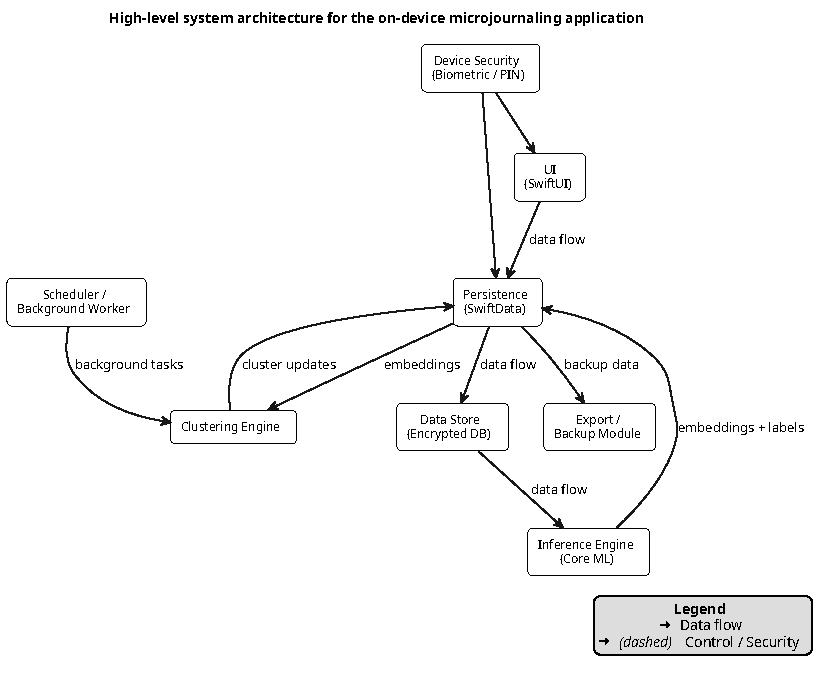
\includegraphics[width=0.85\textwidth]{figures/architecture.pdf}
  \caption{High‑level system architecture showing major components and data flow.}
  \label{fig:architecture}
\end{figure}

\section{Data Flow and Processing Pipeline}
The canonical data flow for a new entry is:

\begin{enumerate}
  \item User creates an entry in the editor and saves it.
  \item The Persistence Layer stores the raw text and metadata.
  \item The Inference Engine generates a semantic embedding and an emotion label for the entry.
  \item The embedding and label are stored alongside the entry.
  \item The Clustering Engine performs an incremental update to cluster assignments.
  \item The UI updates calendar, list, and graph views to reflect the new entry and cluster membership.
\end{enumerate}

A periodic batch job re‑computes clusters and cluster summaries during idle time or when the device is charging.

\section{Use Cases and User Flows}

Table~\ref{tab:use_cases} summarises the four primary use cases.

\begin{table}[h!]
\centering
\caption{Primary use cases.}
\label{tab:use_cases}
\begin{tabular}{p{0.14\textwidth} p{0.30\textwidth} p{0.44\textwidth}}
\hline
\textbf{Use Case} & \textbf{Trigger} & \textbf{System Response} \\
\hline
UC1 Create Entry &
  User fills in Feel, Event, and Action fields and taps Save &
  Entry stored; embedding and emotion label generated on device; cluster assignments updated; calendar, list, and graph views refreshed. \\
\hline
UC2 View Insights &
  User opens the Graph or Insights screen &
  Clusters shown with representative entries and emotion distribution. Tapping a cluster reveals its members. \\
\hline
UC3 Edit Entry &
  User edits an entry created on the same calendar day &
  Text updated; embedding and emotion label recomputed; cluster membership reassigned. \\
\hline
UC4 Delete Entry &
  User deletes an entry &
  Entry soft-deleted and hidden immediately; permanently removed after the three-day grace period. \\
\hline
\end{tabular}
\end{table}

\section{Model Selection and Formats}
Three embedding strategies are implemented behind a common \texttt{EmbeddingService} protocol. all-MiniLM-L6-v2 produces 384-dimensional mean-pooled embeddings and is packaged as a 45\,MB Core ML bundle; it is the default. nomic-embed-text-v1.5 is trained with Matryoshka Representation Learning and produces embeddings at \{64, 128, 256, 512, 768\} dimensions by truncating its output; the default truncation is 256 dimensions and the Core ML package is 274\,MB. Apple NLEmbedding ships with the operating system (zero bundle cost) and produces 512-dimensional vectors. The emotion classifier is MobileBERT fine-tuned for three epochs on GoEmotions, with 28 original labels collapsed to 12 classes (Joy, Sadness, Anger, Fear, Love, Surprise, Disgust, Anxiety, Excitement, Gratitude, Hope, Guilt), packaged as a 99\,MB Core ML bundle. All models are converted using coremltools on a Python workstation.

\section{Clustering Strategy}
The system uses DBSCAN with adaptive parameters. Epsilon is calibrated per corpus as the 10th percentile of pairwise cosine distances; \texttt{minPoints} scales with corpus size between a minimum of 3 and a maximum of 11. For MRL-truncated embeddings, epsilon is further scaled by $\sqrt{d/768}$ to compensate for the compressed distance range at lower dimensions. Each cluster is named by extracting frequent nouns and adjectives from its member entries; if no clear content words emerge, the dominant emotion label is used instead. A background batch job re-runs clustering when the device is idle.

\section{Privacy}
By design, the app does not transmit journal text, embeddings, or cluster metadata off device. No cloud services are involved in any part of the pipeline.

\section{Performance Targets and Testing}
Interactive inference (embedding + emotion classification) should complete within 5 seconds on iPhone 14; incremental cluster membership updates should complete within 2 seconds per new entry. Batch re‑clustering is acceptable to run for several minutes during idle or charging periods. The default model bundle (MiniLM + emotion classifier) targets under 200 MB; the optional Nomic model adds a further 274 MB. The journal database should remain responsive up to 200 MB of stored entries. Testing covers latency, memory, and battery impact on representative devices (iPhone 14 Plus, iPhone 15), and clustering quality via silhouette and ARI metrics on synthetic and anonymized sample data.

\section{Acceptance Criteria}
The prototype is acceptable when FR1--FR7 are implemented and demonstrable, on‑device inference meets the performance targets on the minimum device, data remains local with no off-device transmission, and clustering produces coherent groups visible in the graph view.

\section{Implementation Milestones}
The prototype was developed in five stages:
\begin{enumerate}
  \item \textbf{Scaffolding:} SwiftUI screens for the editor, calendar, list, graph, and settings; SwiftData schema for \texttt{Bit} and \texttt{Cluster} entities.
  \item \textbf{AI pipeline:} Core ML integration for all-MiniLM-L6-v2, nomic-embed-text-v1.5 MRL, Apple NLEmbedding, and MobileBERT emotion classifier; protocol-based \texttt{EmbeddingService} and \texttt{EmotionService} abstractions for interchangeable backends.
  \item \textbf{Clustering engine:} adaptive DBSCAN with epsilon calibration, incremental update on entry save, background batch re-clustering, and TF-IDF cluster naming.
  \item \textbf{Graph visualisation:} force-directed layout, hub-and-spoke edge rendering, pan/zoom gesture handling.
  \item \textbf{Evaluation:} Python benchmarks on STS-B and TwentyNewsgroups; domain validation on 100 labelled journal entries; on-device efficiency benchmark via an in-app measurement tool.
\end{enumerate}

\section{Traceability Matrix}

\begin{table}[h!]
\centering
\caption{Requirement traceability.}
\label{tab:traceability}
\begin{tabular}{p{0.16\textwidth} p{0.36\textwidth} p{0.34\textwidth}}
\hline
\textbf{Requirement} & \textbf{Implementation Component} & \textbf{Acceptance Test} \\
\hline
FR1 Create entry      & SwiftUI editor, SwiftData \texttt{Bit} model          & Save entry; verify text stored and visible in calendar \\
FR2 Entry views       & Calendar, list, graph SwiftUI screens                  & New entry appears in all three views after save \\
FR3 On‑device analysis & \texttt{AIProcessingManager}, Core ML services         & Embedding and emotion label present on \texttt{Bit} after save \\
FR4 Clustering        & \texttt{DBSCANClusterer}, \texttt{Cluster} model        & Entry assigned to cluster; cluster visible in graph \\
FR5 Search/filter     & Repository search API, filter chips                    & Filtering by emotion and cluster returns correct entries \\
FR6 Edit policy       & Editor day-lock logic, embedding update                & Edit updates text, re-runs inference, reassigns cluster \\
FR7 Deletion          & Soft-delete flag, maintenance pass                     & Deleted entry hidden immediately; removed after grace period \\
\hline
\end{tabular}
\end{table}

\section{Open Issues}
The main open issue is SwiftData schema migration: the current implementation wipes stored data on model changes during development. A versioned migration policy is required before any production deployment.

\section{Summary}
This chapter specified the functional and non‑functional requirements, the high‑level architecture, data flow, and acceptance criteria for the on‑device microjournaling system. The next chapter will describe the implementation details, model conversion steps, and the evaluation methodology used to validate the prototype.
